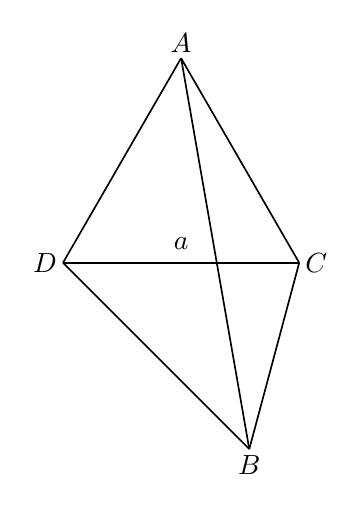
\begin{tikzpicture}[x=1cm,y=1cm,font=\normalsize,
 geometry edge/.style={solid,line width=.6pt},
 geometry mark/.style={solid,line width=.6pt},
 geometry label/.style={font=\normalsize,inner sep=2pt}]
\coordinate (A) at (1.5,5.1321);
\coordinate (D) at (0,2.534);
\coordinate (B) at (2.366,0.168);
\coordinate (C) at (3,2.534);
\draw[geometry edge] (A)--(D);
\draw[geometry edge] (D)--(B);
\draw[geometry edge] (B)--(C);
\draw[geometry edge] (C)--(A);
\draw[geometry edge] (A)--(B);
\draw[geometry edge] (D)--(C);
\node[geometry label,above] at (A) {$A$};
\node[geometry label,left] at (D) {$D$};
\node[geometry label,below] at (B) {$B$};
\node[geometry label,right] at (C) {$C$};
\node at (1.5,2.78) {$a$};
\end{tikzpicture}
